\section{Graph-wide data structure}
\label{sec:graphwide}

Up until now, the main framework we used to solve \cref{prob:shortest-path} has been \cref{alg:portfolio}. Computationally, this offers a lot of potential for saving resources by spending $T^0(\textsc{alg}) = \mathcal O(n^2) \cdot T(\textsc{PortfolioAlg})$ time just once, and then profiting off of smaller $T^q(\textsc{Alg})$. Regarding memory, this can still be costly. The space needed to store the portfolios computed in the preprocessing is $\mathcal O(kn^3)$, since we store $\mathcal O(n^2)$ many portfolio of $k$ paths with a length of up to $n$ vertices. While the average path length might be much less than $n$, even paying for space whose size is quadratic in $n$ can be too expensive.

In this section we thus discuss an approach that uses significantly less space. Consider any portfolio $\mathcal K$ for an instance of \cref{prob:portfolio}. As discussed in \cref{sec:qualitative}, $\mathcal K$ implies a partition $Q(\mathcal K)$ on the cost functions.

Similarly we can deduce a portfolio from some partition $Q$.
\[
$\mathcal K^*(Q) = \left\{\argmin\{\mathbb E[c(e) \mid c \in R]\} \mid R \in Q\right\}$
\]

Note that $K^*(Q)$ is the best portfolio out of all portfolios that induce the identical partition. Thus $\text{cost}(\mathcal K^*(Q(\mathcal K))) \le \text{cost}(\mathcal K)$.

The idea of our algorithm is that we sample $(s,t)$ queries uniformly and compute the $k$-partitions induced by the $k$-portfolios computed for each pair. This gives us a collection of partitions $\mathcal Q$. These we aggregate to a single partition $\overline Q$ that is representative of $\mathcal Q$.

Given $\overline Q$ we can seperate $G$ into $k$ non-stochastic graphs, each having the mean edge costs of one of the sets in $\overline Q$. We can now proceed with using any known algorithm that can preprocess fixed graphs and answer shortest-path queries fast. A field of research that aims to solve such problems tries to introduce hierarchies to the graph nodes or edges, only precomputing paths between vertices in the same level.

For this project, there was not enough time left to properly investigate the results such an algorithm would yield.
In order for it to work there has to exist some partition of the cost functions, that is able to represent the different traffic scenarios throughout the entire graph. If for every $(s,t)$ query we find entirely new partitions, then there might not be any way to aggregate them.

Assuming a representative partition of the cost functions can be found it would be interesting to visualise that partition on a calendar-like chart as in \cref{fig:april}. Is there more to it than just finding the rushhours, night times and weekends?

We ran some first experiments trying to find some partition $\overline Q$. For an increasing number of $q=|\mathcal Q|$ we ran 20 experiments each, ending up with a $\overline{Q}$ for each. We aggregated the sets of partitions using the k-medoidsalgorithm and the hamming distance between two partitions. If there was some representative partition emerging, then those $\overline{Q}$ should be similar.
We are plotting the hamming distances between these in \cref{fig:}. As one can see the obtained partitions from re-running experiments differ quite strongly, hinting towards the difficulty of finding meaningful graph-wide cost function partitions. For reference, the hamming distance between uniformly random partition has an expected value of 2880, which is two thirds of the number of cost functions in \cref{shanghai}. There is a clear downwards trend as $q$ increases, so one would have to definitely study what happens for clearly larger amounts of $(s,t)$ queries. Maybe more representative data can be found.

\begin{figure}
    \centering
    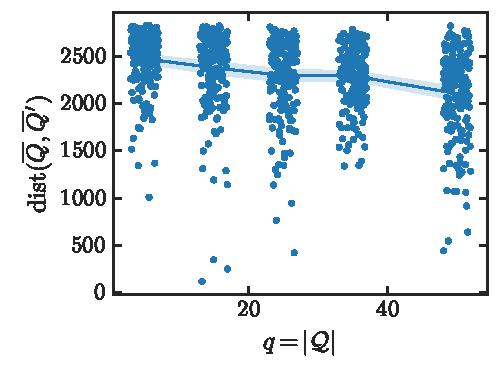
\includegraphics{figures/clustering_distances.pdf}
\caption{Pairwise distances between 20 ``representative'' partitions obtained from a collection of $q$ partitions for different values of $q$.}
\label{fig:1749g_vs_m}
\end{figure}

